\documentclass{article}

\usepackage[utf8]{inputenc}
\usepackage{fancyhdr}
\usepackage{float}
\usepackage{tikz}
\usepackage{graphicx}
\usepackage{url}
\usetikzlibrary{arrows}
\usetikzlibrary{positioning}
\pagestyle{fancy}
\graphicspath{{img/}}
\renewcommand\thepart{\Alph{part}}

\newcommand\TODO[1]{\textcolor{red}{TODO:#1}}
\newcommand\todo[1]{\TODO{#1}}

\title{Homework Module: A Controller for Swarm Behaviour in Webots}

\lhead{Homework Module \#1}
\rhead{IT3708 - Subsymbolic Methods in AI}

\author{
    Aleksander Burkow \\
    Sigve Sebstian Farstad \\
    Emil Grønnbeck
}

\begin{document}

\maketitle
\thispagestyle{empty}

\abstract{
This report presents a solution for Homework Module \#1 of IT3708, spring 2014 at NTNU.
The purpose of the homework module is to ``understand swarm behaviour by implementing a controller for box pushing task in Webots''.~\cite{assignment}
}

\newpage

\setcounter{page}{1}

\part{The Proposed System}

\section{Description}

\begin{figure}[H]
\centering
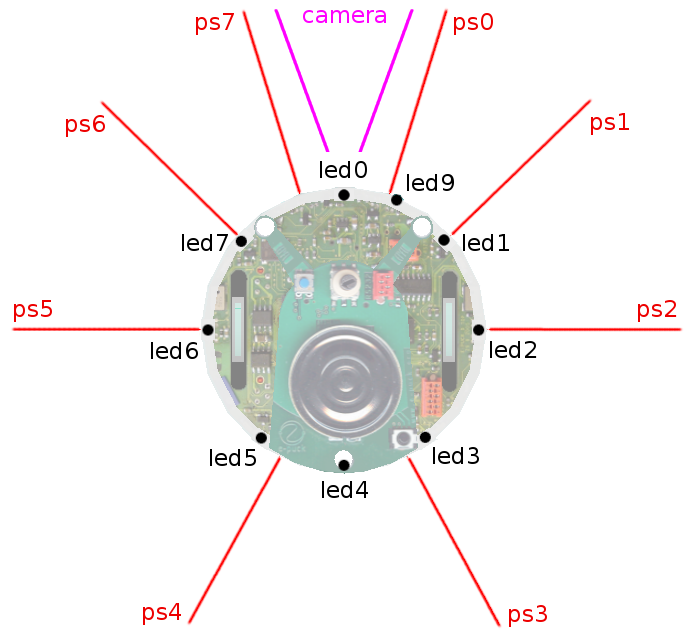
\includegraphics[scale=0.2]{e-puck_sensors_and_leds.png}
\caption{E-puck robot with all sensors}
\end{figure}

\subsection{Swarm intelligence in nature}



\subsection{Brooks Architecture}
The system we implemented is based on an AI concept called subsumption architecture.
Subsumption architecture was first described by Rodney Brooks in the mid 80's.
The idea behind subsumption architecture came from insects.
Insects though with relatively little computational power, is able to walk, avoid obstacles, and make desicions faster than any robot created.
The architecture is divided into layers called: "the levels of competence".
Each layer is  independent of each other, where the higher levels are capable of overriding the lower[1].
The highest stimulated behaviour is acted upon [2]

\subsection{Our implementation}
We divided our "levels of competence" into six independent behaviours; Wander, Avoid obstacles, Converge, Retrieve, and Reposition.
The lower levels have a higher priority and are able to override the higher ones.
\begin{figure}[H]
\centering
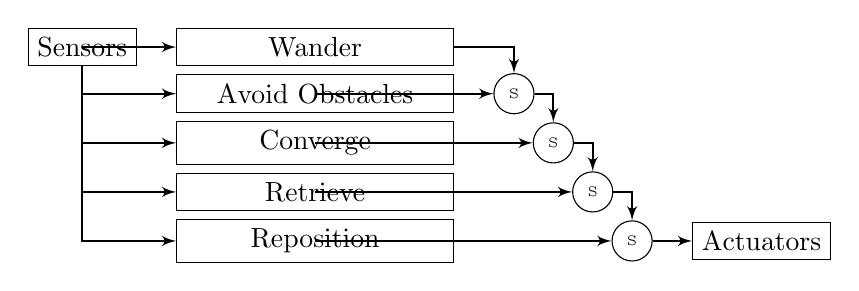
\begin{tikzpicture}

\tikzstyle{behaviour}=[draw, minimum width=10em, right=5mm of sensors]
\tikzstyle{line}=[draw, thick, -latex']
\tikzstyle{subsumption}=[draw, circle]

\node[draw] (sensors) {Sensors};

\node[behaviour] (wander) {Wander};
\node[behaviour, below=1mm of wander] (avoid_obstacles) {Avoid Obstacles};
\node[behaviour, below=1mm of avoid_obstacles] (converge) {Converge};
\node[behaviour, below=1mm of converge] (retrieve) {Retrieve};
\node[behaviour, below=1mm of retrieve] (reposition) {Reposition};

\node[subsumption, right=5mm of avoid_obstacles] (avoid_obstacles_subsumption) {\tiny S};
\node[subsumption, right=10mm of converge] (converge_subsumption) {\tiny S};
\node[subsumption, right=15mm of retrieve] (retrieve_subsumption) {\tiny S};
\node[subsumption, right=20mm of reposition] (reposition_subsumption) {\tiny S};
\node[draw, right=5mm of reposition_subsumption] (actuators) {Actuators};

\path[line] (sensors) |- (wander);
\path[line] (sensors) |- (avoid_obstacles);
\path[line] (sensors) |- (converge);
\path[line] (sensors) |- (retrieve);
\path[line] (sensors) |- (reposition);

\path[line] (avoid_obstacles) |- (avoid_obstacles_subsumption);
\path[line] (converge) |- (converge_subsumption);
\path[line] (retrieve) |- (retrieve_subsumption);
\path[line] (reposition) |- (reposition_subsumption);

\path[line] (wander) -| (avoid_obstacles_subsumption);
\path[line] (avoid_obstacles_subsumption) -| (converge_subsumption);
\path[line] (converge_subsumption) -| (retrieve_subsumption);
\path[line] (retrieve_subsumption) -| (reposition_subsumption);
\path[line] (reposition_subsumption) -- (actuators);

\end{tikzpicture}
\caption{The subsumption architecture of the proposed system.}
\label{figure:subsumption}
\end{figure}


\subsubsection{Wander}
Wander is our default behaviour, it basically tells the robot to run straight forward.
It has no stimulus, when no other behaviour is stimulated, the robot acts on this behaviour

\subsubsection{Avoid obstacles}
The avoid obstacles behaviour is triggered when the epucks proximity sensors rise above a certain threshold, indicating that it's close to or about to hit a wall.

The rotational angle of the differential wheels is then set proportional to the difference between the amount of obstacles on either side of the robot, such that it turns away from the observed obstacles.

The closer the wall is on the right side, the harder the epuck will turn to the left, and vice versa.

\subsubsection{Converge}
The converge behaviour is triggered when the sum of the epucks light sensors rise above a certain threshold, indicating that food is nearby.

The rotational angle of the differential wheels is set in proportion to the amount of light on either side, such that the robot heads towards the light.

\subsubsection{Retrieve}
The retrieve behaviour is triggered when the epuck detects that food is straight ahead, but that it's not yet close enough to begin retrieval.

The behaviour will try to align the robot with the surface normal of the object, so that it's driving directly into the food for maximum force

\subsubsection{Reposition}
The reposition behaviour is enabled when the epuck has found the food, and is trying to bring it home.

There's a chance that pucks may be hindering progress by pushing o, and that some of the pucks will need to realign themselves if they wish to return home triumphantly with food.
We solved this problem as follows:

When an epuck realizes it's driving into the food, it will blindly drive straight ahead


 and a realign is needed to get anywhere at all.
 Our reposition behaviour implements a stateless way to realign the epuck after some time has passed.

\section{Simulation Results}
blabalbal
\begin{table}[H]
\centering
\begin{tabular}{ c | c | p{5cm}}
\hline No & Time & Notes \\ \hline
 1 & 42:56 &  \\ \hline
 2 & 38:21 & \\ \hline
 3 & 33:54 & Close to optimal run \\ \hline
4 & - & Two robots got stuck between the box and the wall. Therefore the robots was not able to finish the objective \\ \hline
5 & 36:35 & \\ \hline
6	& 52:13 & The robots did change pushing direction in the middle of the simulation \\ \hline
7 & 59:81 & \\ \hline
8 & 52:83 & \\ \hline
9 & 3:32:01 &  The robots divided into two groups and pushed from opposite sides \\ \hline
10 & 1:42:84 & The robots divided into two groups and pushed from oppsite sides, though the stagnation got solved earlier than simulation 9 \\
\end{tabular}
\caption{One box problem runs}
\end{table}


\begin{table}
\centering
\begin{tabular}{ l | r}
\hline Number of runs & Avg. Time \\ \hline
9 & ?:??:?? \\
\end{tabular}
\caption{ Average time of One box problem runs}
\end{table}


\subsection{Observed weaknesses}
\part{An Improved System}

\section{Description}
\section{Simulation Results}
\part{A More Advanced Architecture}

\section{Description}
\newpage
\section{Simulation Results}
\begin{table}[H]
\centering
\begin{tabular}{ c | c | p{5cm}}
\hline No & Time & Notes \\ \hline

1 & 5:01:96 & The robots were trying to push a box that allready was retrieved \\ \hline
2 & 2:38:43 & \\ \hline
3 & 5:20:45 & Same as simulation number 1 \\ \hline
4


\end{tabular}
\end{table}


\newpage
%\part{Appendix}
%\begin{figure}[H]
%\centering
\todo{Include the picture in the repo}
%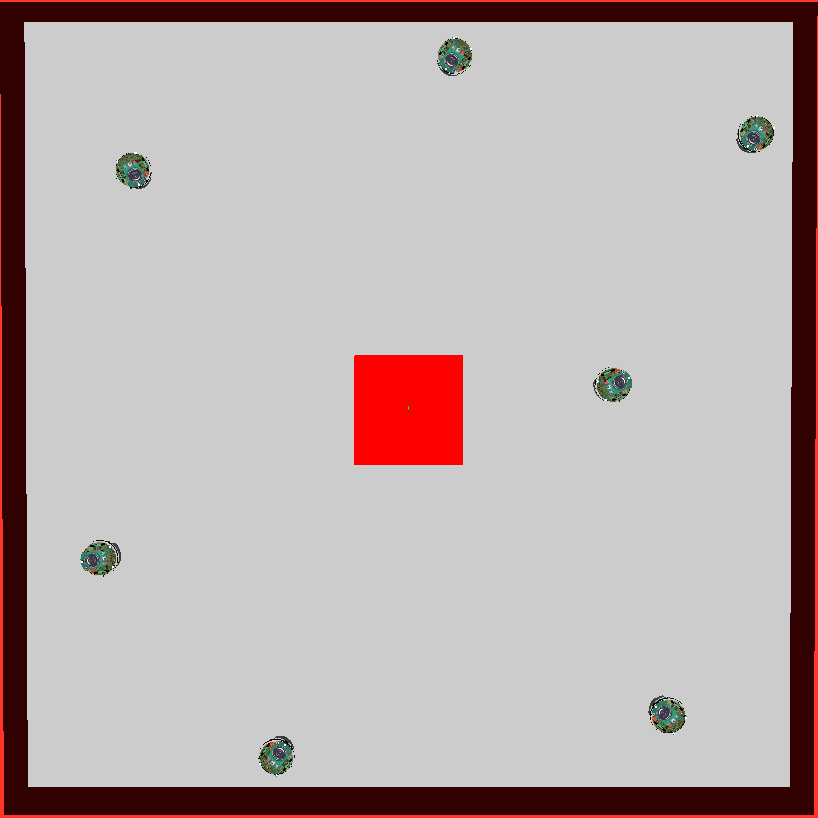
\includegraphics[scale=0.5]{one-box-world.png}
%\caption{World used in the simulation for Table 1}
%\end{figure}

\newpage
\part{References}
[1]http://mwarnerwu.wordpress.com/research/subsumption-architecture/
[2]Jannik Berg and Camilla Haukenes Karud. Swarm intelligence in bio-inspired robotics. PhD thesis,
Norwegian University of Science and Technology, 2011.

\bibliography{reference-library}
\bibliographystyle{plain}
\nocite{*}

\end{document}
